\chapter{Einstieg in das Projekt}
\label{ch:planung}

Bevor mit der Implementierung der \ac{KI} begonnen werden konnte, mussten zuerst noch einige andere Punkte geklärt
\bzw erledigt werden.
Diese ersten Schritte werden im Folgenden erläutert.

\section{Auswahl der Programmiersprache}
\label{sec:auswahl-programmiersprache}

Zu Beginn war zu klären, mit welcher Programmiersprache dieser Lösungsvorschlag umgesetzt werden soll.
Die Wahl ist dabei schnell auf Python gefallen, obwohl beide Gruppenmitglieder hiermit noch keinerlei Erfahrung
aufweisen konnten.
Der Grund für diese Entscheidung liegt neben dem starken Interessen an dem Kennenlernen einer neuen Programmiersprache
auch an der bereits sehr hohen und immer noch steigenden Popularität der Programmiersprache und der damit verbundenen
zukünftigen Wichtigkeit. \Vgl{tiobe} \Vgl{pypl}
Hinzu kommt, dass wir vor Beginn der Implementierung anhand der Aufgabenstellung das Potenzial für den Einsatz von
Machine Learning gesehen haben und Python in diesem Bereich oft empfohlen wird. \Vgl{springboard} \Vgl{towardsscience}

\section{Erstellung eines lauffähigen Projekts}
\label{sec:erstellung-projekt}

Damit unsere zu implementierende Lösung auch ausgeführt und manuell getestet werden konnte, war es zunächst notwendig,
ein minimales, ausführbares Projekt aufzusetzen.

\subsection{Einsatz von Poetry als Build-Tool}
\label{subsec:poetry}

Ein einfacher Weg, um Abhängigkeiten in Python zu verwalten, ist, eine Datei mit dem Namen \Code{requirements.txt} zu
verwenden und in dieser die eingesetzten Bibliotheken aufzulisten. \Vgl{requirements-txt}
Wir haben uns allerdings für die Verwendung von Poetry als vollständiges Build-Tool entschieden, da dieses zum Einen
sehr einfach zum Einstieg ist und simple Kommandozeilen-Befehle bereitstellt, zum Anderen aber auch weitere Funktionen
wie das Ausführen von Tests und Erstellen eines fertigen Pakets anbietet und die Auflösung komplexerer Abhängigkeiten
von Paketen durch dieses Tool sehr gut funktioniert. \Vgl{poetry}

\subsection{Entwicklung eines Dockerfile}
\label{subsec:dockerfile}

Zum Start haben wir ein minimales Python-Skript erstellt, das lediglich die an den Docker-Container übergebenen
Parameter für die Server-URL und den API-Key ausgibt.
Zwar mussten bis hierhin noch keine Abhängigkeiten hinzugefügt werden, aber bei der Konzeption des Dockerfiles sollte
bereits die Installation zusätzlicher Bibliotheken berücksichtigt werden.
Mit der Nutzung des Standard-Python-Containers von Docker Hub \Vgl{python-dockerhub} wird bereits ein vorgefertigter
Container bereitgestellt, in dem Python und Pip installiert ist.
Bei Pip handelt es sich um "`ein rekursives Akronym für Pip Installs Python und ist das Standardverwaltungswerkzeug
für Python-Module"' \Vgl{pip}.
Mittels diesem Tool wird die Installation von Poetry durchgeführt.
Poetry wiederum bietet anschließend die Möglichkeit, die verwalteten Abhängigkeiten in Form einer
\texttt{requirements.txt}-Datei zu exportieren, welche dann von Pip eingelesen werden kann, um die Bibliotheken zu
installieren. \\

Letztendlich wurde ein Dockerfile entworfen, welches die in \Listing{lst:dockerfile} dargestellten Befehle enthält.
Die Umgebungsvariable \Code{TERM} wird gesetzt, um eine farbliche Ausgabe in der Konsole zu ermöglichen.
Auf die Parameter zum Start der Anwendung wird in \Kapitel{ch:benutzerhandbuch} eingegangen.
Bei der Erstellung wurden die von Docker vorgeschlagenen Best Practices \Vgl{docker-best-practices} umgesetzt.

\lstinputlisting[label=lst:dockerfile,language=Java,caption=Dockerfile zum Erstellen eines lauffähigen Containers]
{../Dockerfile}

\section{Nachstellung des Spiels}
\label{sec:nachstellung-spiel}

Um die zu entwickelnde \ac{KI} ohne die Server-Verbindung manuell testen zu können, haben wir bei der Implementierung
damit begonnen, die Spiellogik nachzustellen.
Dazu haben wir nach Erhalt des API-Keys anhand der bereitgestellten Dokumentation und der Möglichkeit, das Spiel in
einer Online-Version im Browser testen zu können, begonnen, die Spiellogik zu analysieren. \\

Diese Logik ist relativ einfach nachzuvollziehen.
Nachdem alle Spieler ihre Aktion an den Server gesendet haben, wird jede Aktion eines Spielers in einer Runde zeitgleich
ausgeführt.
Trifft der Spieler während seiner Aktion auf ein bereits belegtes Feld, so verliert dieser das Spiel, bewegt sich
aber noch so viele Felder weiter vorwärts, wie es seine Geshwindigkeit und Richtung normalerweise bewirkt hätte.
Verhindert werden können solche Kollisionen mithilfe eines Sprungs, der bei entsprechendem Tempo automatisch in jeder
sechsten Runde des Spiels ausgeführt wird. \\

Wir haben diese Logik, auf die wir später noch genauer eingehen werden und die bei der Implementierung der \ac{KI}s
wiederverwendet werden konnte, in einer Klasse \Code{GameService} implementiert.
Zum Testen haben wir zwei verschiedene Oberflächen entwickelt.
Zum einen kann das Spielfeld nach jeder Runde auf der Konsole ausgegeben werden.
Dazu wird das Spielfeld als Tabelle dargestellt und in den Zellen, in denen sich ein Spieler befindet, wird dessen
Spieler-ID angezeigt.
Diese Darstellung wird in der \Abbildung{fig:KonsolenOberflaeche} verdeutlicht.

\begin{figure}[htb]
\centering
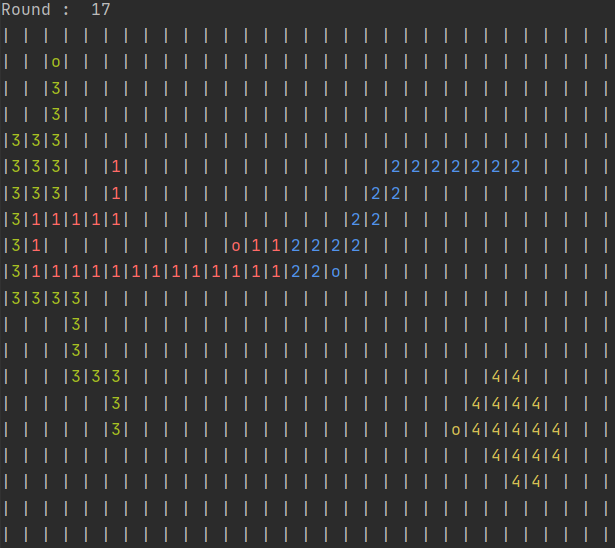
\includegraphics[width=0.6\textwidth]{Bilder/KonsolenOberflaeche.png}
\caption{Darstellung der Oberfläche in der Konsole}
\label{fig:KonsolenOberflaeche}
\end{figure}

Zum anderen gibt es auch die Möglichkeit, das Spiel auf einer grafischen Oberfläche zu spielen, die mittels PyGame
\Vgl{pygame} entworfen wurde.
Jedem Spieler wird dabei zu Spielbeginn eine Farbe zugeordnet, um die verschiedenen Spieler auseinanderhalten zu können.
Ein Spiel mit grafischer Oberfläche wird in \Abbildung{fig:GrafischeOberflaeche} gezeigt.

\begin{figure}[htb]
\centering
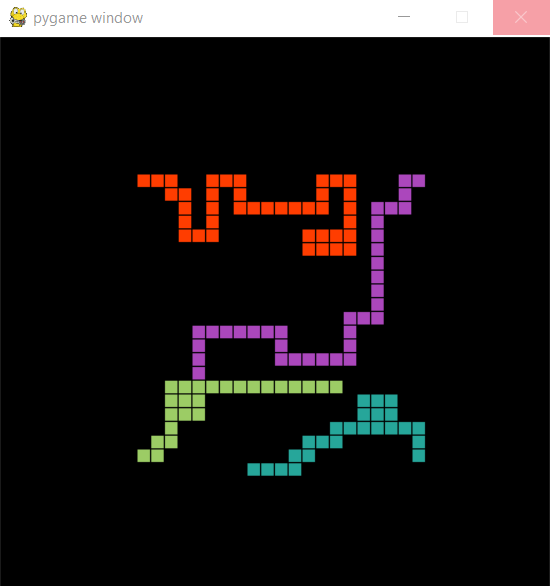
\includegraphics[width=0.5\textwidth]{Bilder/GrafischeOberflaeche.png}
\caption{Darstellung der grafischen Oberfläche mit PyGame}
\label{fig:GrafischeOberflaeche}
\end{figure}